\documentclass[twoside]{book}

% Packages required by doxygen
\usepackage{fixltx2e}
\usepackage{calc}
\usepackage{doxygen}
\usepackage[export]{adjustbox} % also loads graphicx
\usepackage{graphicx}
\usepackage[utf8]{inputenc}
\usepackage{makeidx}
\usepackage{multicol}
\usepackage{multirow}
\PassOptionsToPackage{warn}{textcomp}
\usepackage{textcomp}
\usepackage[nointegrals]{wasysym}
\usepackage[table]{xcolor}

% Font selection
\usepackage[T1]{fontenc}
\usepackage[scaled=.90]{helvet}
\usepackage{courier}
\usepackage{amssymb}
\usepackage{sectsty}
\renewcommand{\familydefault}{\sfdefault}
\allsectionsfont{%
  \fontseries{bc}\selectfont%
  \color{darkgray}%
}
\renewcommand{\DoxyLabelFont}{%
  \fontseries{bc}\selectfont%
  \color{darkgray}%
}
\newcommand{\+}{\discretionary{\mbox{\scriptsize$\hookleftarrow$}}{}{}}

% Page & text layout
\usepackage{geometry}
\geometry{%
  a4paper,%
  top=2.5cm,%
  bottom=2.5cm,%
  left=2.5cm,%
  right=2.5cm%
}
\tolerance=750
\hfuzz=15pt
\hbadness=750
\setlength{\emergencystretch}{15pt}
\setlength{\parindent}{0cm}
\setlength{\parskip}{3ex plus 2ex minus 2ex}
\makeatletter
\renewcommand{\paragraph}{%
  \@startsection{paragraph}{4}{0ex}{-1.0ex}{1.0ex}{%
    \normalfont\normalsize\bfseries\SS@parafont%
  }%
}
\renewcommand{\subparagraph}{%
  \@startsection{subparagraph}{5}{0ex}{-1.0ex}{1.0ex}{%
    \normalfont\normalsize\bfseries\SS@subparafont%
  }%
}
\makeatother

% Headers & footers
\usepackage{fancyhdr}
\pagestyle{fancyplain}
\fancyhead[LE]{\fancyplain{}{\bfseries\thepage}}
\fancyhead[CE]{\fancyplain{}{}}
\fancyhead[RE]{\fancyplain{}{\bfseries\leftmark}}
\fancyhead[LO]{\fancyplain{}{\bfseries\rightmark}}
\fancyhead[CO]{\fancyplain{}{}}
\fancyhead[RO]{\fancyplain{}{\bfseries\thepage}}
\fancyfoot[LE]{\fancyplain{}{}}
\fancyfoot[CE]{\fancyplain{}{}}
\fancyfoot[RE]{\fancyplain{}{\bfseries\scriptsize Generated by Doxygen }}
\fancyfoot[LO]{\fancyplain{}{\bfseries\scriptsize Generated by Doxygen }}
\fancyfoot[CO]{\fancyplain{}{}}
\fancyfoot[RO]{\fancyplain{}{}}
\renewcommand{\footrulewidth}{0.4pt}
\renewcommand{\chaptermark}[1]{%
  \markboth{#1}{}%
}
\renewcommand{\sectionmark}[1]{%
  \markright{\thesection\ #1}%
}

% Indices & bibliography
\usepackage{natbib}
\usepackage[titles]{tocloft}
\setcounter{tocdepth}{3}
\setcounter{secnumdepth}{5}
\makeindex

% Hyperlinks (required, but should be loaded last)
\usepackage{ifpdf}
\ifpdf
  \usepackage[pdftex,pagebackref=true]{hyperref}
\else
  \usepackage[ps2pdf,pagebackref=true]{hyperref}
\fi
\hypersetup{%
  colorlinks=true,%
  linkcolor=blue,%
  citecolor=blue,%
  unicode%
}

% Custom commands
\newcommand{\clearemptydoublepage}{%
  \newpage{\pagestyle{empty}\cleardoublepage}%
}

\usepackage{caption}
\captionsetup{labelsep=space,justification=centering,font={bf},singlelinecheck=off,skip=4pt,position=top}

%===== C O N T E N T S =====

\begin{document}

% Titlepage & ToC
\hypersetup{pageanchor=false,
             bookmarksnumbered=true,
             pdfencoding=unicode
            }
\pagenumbering{alph}
\begin{titlepage}
\vspace*{7cm}
\begin{center}%
{\Large T\+Pigl }\\
\vspace*{1cm}
{\large Generated by Doxygen 1.8.13}\\
\end{center}
\end{titlepage}
\clearemptydoublepage
\pagenumbering{roman}
\tableofcontents
\clearemptydoublepage
\pagenumbering{arabic}
\hypersetup{pageanchor=true}

%--- Begin generated contents ---
\chapter{Namespace Index}
\section{Packages}
Here are the packages with brief descriptions (if available)\+:\begin{DoxyCompactList}
\item\contentsline{section}{\hyperlink{namespace_t_pigl}{T\+Pigl} }{\pageref{namespace_t_pigl}}{}
\item\contentsline{section}{\hyperlink{namespace_t_pigl_1_1_properties}{T\+Pigl.\+Properties} }{\pageref{namespace_t_pigl_1_1_properties}}{}
\end{DoxyCompactList}

\chapter{Hierarchical Index}
\section{Class Hierarchy}
This inheritance list is sorted roughly, but not completely, alphabetically\+:\begin{DoxyCompactList}
\item Application\begin{DoxyCompactList}
\item \contentsline{section}{T\+Pigl.\+App}{\pageref{class_t_pigl_1_1_app}}{}
\end{DoxyCompactList}
\item \contentsline{section}{T\+Pigl.\+vector\+Helper}{\pageref{class_t_pigl_1_1vector_helper}}{}
\item Window\begin{DoxyCompactList}
\item \contentsline{section}{T\+Pigl.\+Main\+Window}{\pageref{class_t_pigl_1_1_main_window}}{}
\end{DoxyCompactList}
\end{DoxyCompactList}

\chapter{Class Index}
\section{Class List}
Here are the classes, structs, unions and interfaces with brief descriptions\+:\begin{DoxyCompactList}
\item\contentsline{section}{\hyperlink{class_t_pigl_1_1_app}{T\+Pigl.\+App} \\*Logique d\textquotesingle{}interaction pour App.\+xaml }{\pageref{class_t_pigl_1_1_app}}{}
\item\contentsline{section}{\hyperlink{class_t_pigl_1_1_main_window}{T\+Pigl.\+Main\+Window} }{\pageref{class_t_pigl_1_1_main_window}}{}
\item\contentsline{section}{\hyperlink{class_t_pigl_1_1vector_helper}{T\+Pigl.\+vector\+Helper} }{\pageref{class_t_pigl_1_1vector_helper}}{}
\end{DoxyCompactList}

\chapter{File Index}
\section{File List}
Here is a list of all files with brief descriptions\+:\begin{DoxyCompactList}
\item\contentsline{section}{D\+:/git/tp/\hyperlink{_app_8xaml_8cs}{App.\+xaml.\+cs} }{\pageref{_app_8xaml_8cs}}{}
\item\contentsline{section}{D\+:/git/tp/\hyperlink{_main_window_8xaml_8cs}{Main\+Window.\+xaml.\+cs} }{\pageref{_main_window_8xaml_8cs}}{}
\item\contentsline{section}{D\+:/git/tp/\hyperlink{_settings_8cs}{Settings.\+cs} }{\pageref{_settings_8cs}}{}
\item\contentsline{section}{D\+:/git/tp/\hyperlink{vector_helper_8cs}{vector\+Helper.\+cs} }{\pageref{vector_helper_8cs}}{}
\end{DoxyCompactList}

\chapter{Namespace Documentation}
\hypertarget{namespace_t_pigl}{}\section{T\+Pigl Namespace Reference}
\label{namespace_t_pigl}\index{T\+Pigl@{T\+Pigl}}
\subsection*{Namespaces}
\begin{DoxyCompactItemize}
\item 
namespace \hyperlink{namespace_t_pigl_1_1_properties}{Properties}
\end{DoxyCompactItemize}
\subsection*{Classes}
\begin{DoxyCompactItemize}
\item 
class \hyperlink{class_t_pigl_1_1_app}{App}
\begin{DoxyCompactList}\small\item\em Logique d\textquotesingle{}interaction pour App.\+xaml \end{DoxyCompactList}\item 
class \hyperlink{class_t_pigl_1_1_main_window}{Main\+Window}
\item 
class \hyperlink{class_t_pigl_1_1vector_helper}{vector\+Helper}
\end{DoxyCompactItemize}

\hypertarget{namespace_t_pigl_1_1_properties}{}\section{T\+Pigl.\+Properties Namespace Reference}
\label{namespace_t_pigl_1_1_properties}\index{T\+Pigl.\+Properties@{T\+Pigl.\+Properties}}
\subsection*{Classes}
\begin{DoxyCompactItemize}
\item 
class {\bfseries Settings}
\end{DoxyCompactItemize}

\chapter{Class Documentation}
\hypertarget{class_t_pigl_1_1_app}{}\section{T\+Pigl.\+App Class Reference}
\label{class_t_pigl_1_1_app}\index{T\+Pigl.\+App@{T\+Pigl.\+App}}


Logique d\textquotesingle{}interaction pour App.\+xaml  


Inheritance diagram for T\+Pigl.\+App\+:\begin{figure}[H]
\begin{center}
\leavevmode
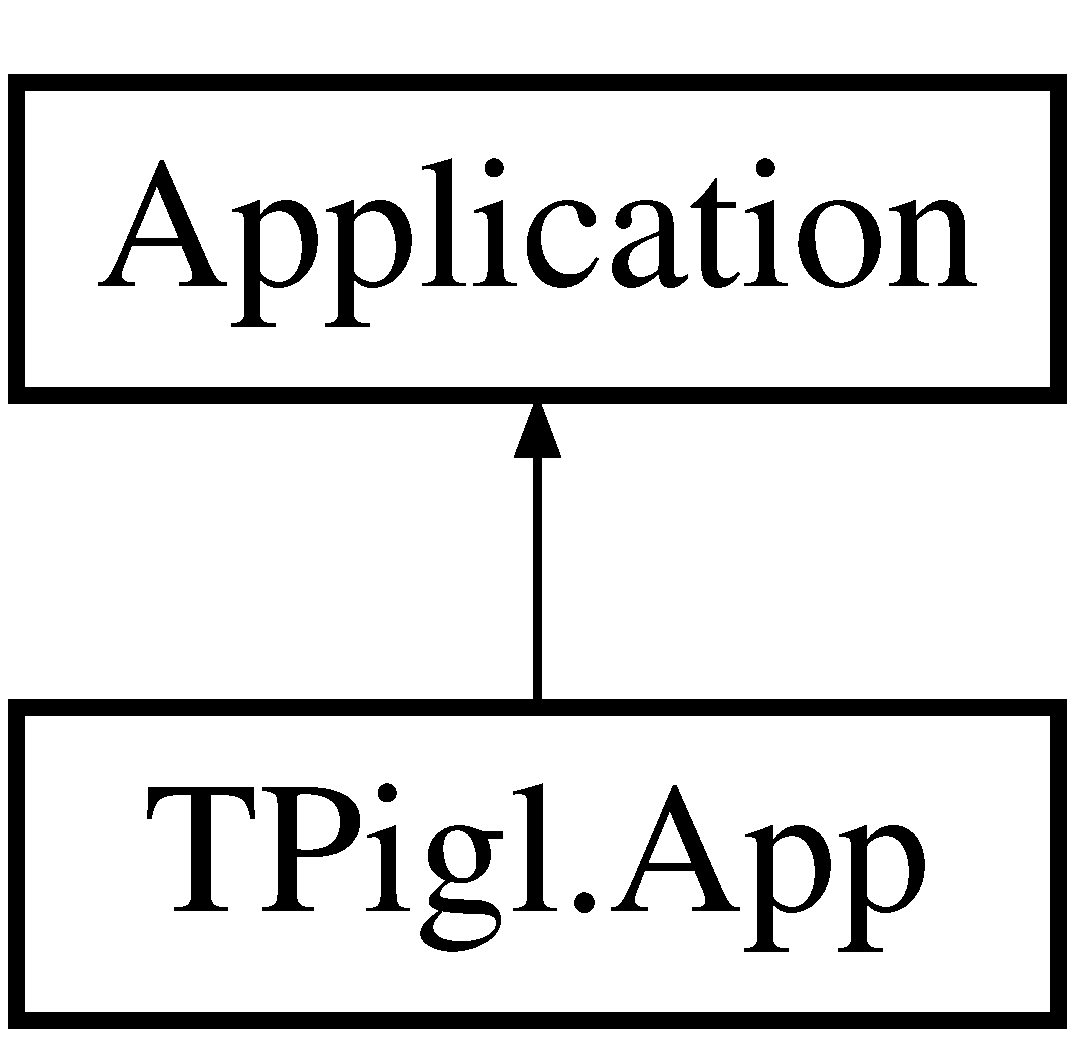
\includegraphics[height=2.000000cm]{class_t_pigl_1_1_app}
\end{center}
\end{figure}


\subsection{Detailed Description}
Logique d\textquotesingle{}interaction pour App.\+xaml 



The documentation for this class was generated from the following file\+:\begin{DoxyCompactItemize}
\item 
D\+:/git/tp/\hyperlink{_app_8xaml_8cs}{App.\+xaml.\+cs}\end{DoxyCompactItemize}

\hypertarget{class_t_pigl_1_1_main_window}{}\section{T\+Pigl.\+Main\+Window Class Reference}
\label{class_t_pigl_1_1_main_window}\index{T\+Pigl.\+Main\+Window@{T\+Pigl.\+Main\+Window}}
Inheritance diagram for T\+Pigl.\+Main\+Window\+:\begin{figure}[H]
\begin{center}
\leavevmode
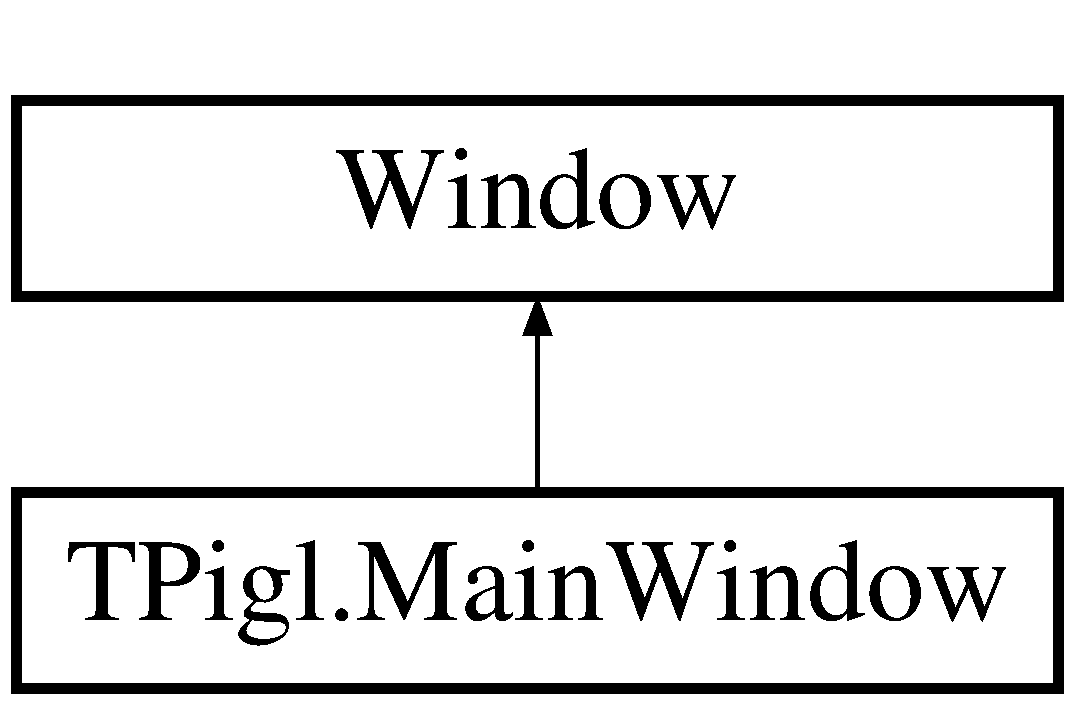
\includegraphics[height=2.000000cm]{class_t_pigl_1_1_main_window}
\end{center}
\end{figure}
\subsection*{Public Member Functions}
\begin{DoxyCompactItemize}
\item 
\hyperlink{class_t_pigl_1_1_main_window_ab295945df11be4072372e118ce1d0d9b}{Main\+Window} ()
\item 
void \hyperlink{class_t_pigl_1_1_main_window_a1f2d24cc72d41c74fbe54266b45ef264}{my\+Text\+Box\+\_\+\+Text\+Changed} (object sender, Text\+Changed\+Event\+Args e)
\item 
void \hyperlink{class_t_pigl_1_1_main_window_a492d481e2c1d21f17abfc8c5dc2eac5b}{set\+\_\+result} (int\mbox{[}$\,$\mbox{]} tab)
\begin{DoxyCompactList}\small\item\em méthode qui permet de calculer le vecteur en sortie après une opétion (tri, inversion ...) \end{DoxyCompactList}\end{DoxyCompactItemize}


\subsection{Constructor \& Destructor Documentation}
\mbox{\Hypertarget{class_t_pigl_1_1_main_window_ab295945df11be4072372e118ce1d0d9b}\label{class_t_pigl_1_1_main_window_ab295945df11be4072372e118ce1d0d9b}} 
\index{T\+Pigl\+::\+Main\+Window@{T\+Pigl\+::\+Main\+Window}!Main\+Window@{Main\+Window}}
\index{Main\+Window@{Main\+Window}!T\+Pigl\+::\+Main\+Window@{T\+Pigl\+::\+Main\+Window}}
\subsubsection{\texorpdfstring{Main\+Window()}{MainWindow()}}
{\footnotesize\ttfamily T\+Pigl.\+Main\+Window.\+Main\+Window (\begin{DoxyParamCaption}{ }\end{DoxyParamCaption})}



\subsection{Member Function Documentation}
\mbox{\Hypertarget{class_t_pigl_1_1_main_window_a1f2d24cc72d41c74fbe54266b45ef264}\label{class_t_pigl_1_1_main_window_a1f2d24cc72d41c74fbe54266b45ef264}} 
\index{T\+Pigl\+::\+Main\+Window@{T\+Pigl\+::\+Main\+Window}!my\+Text\+Box\+\_\+\+Text\+Changed@{my\+Text\+Box\+\_\+\+Text\+Changed}}
\index{my\+Text\+Box\+\_\+\+Text\+Changed@{my\+Text\+Box\+\_\+\+Text\+Changed}!T\+Pigl\+::\+Main\+Window@{T\+Pigl\+::\+Main\+Window}}
\subsubsection{\texorpdfstring{my\+Text\+Box\+\_\+\+Text\+Changed()}{myTextBox\_TextChanged()}}
{\footnotesize\ttfamily void T\+Pigl.\+Main\+Window.\+my\+Text\+Box\+\_\+\+Text\+Changed (\begin{DoxyParamCaption}\item[{object}]{sender,  }\item[{Text\+Changed\+Event\+Args}]{e }\end{DoxyParamCaption})}

\mbox{\Hypertarget{class_t_pigl_1_1_main_window_a492d481e2c1d21f17abfc8c5dc2eac5b}\label{class_t_pigl_1_1_main_window_a492d481e2c1d21f17abfc8c5dc2eac5b}} 
\index{T\+Pigl\+::\+Main\+Window@{T\+Pigl\+::\+Main\+Window}!set\+\_\+result@{set\+\_\+result}}
\index{set\+\_\+result@{set\+\_\+result}!T\+Pigl\+::\+Main\+Window@{T\+Pigl\+::\+Main\+Window}}
\subsubsection{\texorpdfstring{set\+\_\+result()}{set\_result()}}
{\footnotesize\ttfamily void T\+Pigl.\+Main\+Window.\+set\+\_\+result (\begin{DoxyParamCaption}\item[{int \mbox{[}$\,$\mbox{]}}]{tab }\end{DoxyParamCaption})}



méthode qui permet de calculer le vecteur en sortie après une opétion (tri, inversion ...) 



The documentation for this class was generated from the following file\+:\begin{DoxyCompactItemize}
\item 
D\+:/git/tp/\hyperlink{_main_window_8xaml_8cs}{Main\+Window.\+xaml.\+cs}\end{DoxyCompactItemize}

\hypertarget{class_t_pigl_1_1vector_helper}{}\section{T\+Pigl.\+vector\+Helper Class Reference}
\label{class_t_pigl_1_1vector_helper}\index{T\+Pigl.\+vector\+Helper@{T\+Pigl.\+vector\+Helper}}
\subsection*{Public Member Functions}
\begin{DoxyCompactItemize}
\item 
void \hyperlink{class_t_pigl_1_1vector_helper_a9447a1390b9a09ade0d252d8c21a901a}{tri} (int\mbox{[}$\,$\mbox{]} tab)
\begin{DoxyCompactList}\small\item\em la méthode tri permet de trier le vecteur par ordre croissant \end{DoxyCompactList}\item 
void \hyperlink{class_t_pigl_1_1vector_helper_aef84f14c086e1aae4f9446309ba0a1b8}{somme} (int\mbox{[}$\,$\mbox{]} tab1, int\mbox{[}$\,$\mbox{]} tab2)
\begin{DoxyCompactList}\small\item\em la méthode somme permet de sommer deux vecteurs \end{DoxyCompactList}\item 
void \hyperlink{class_t_pigl_1_1vector_helper_a90f5b534a7762117ce843ce79be2fced}{inverser} (int\mbox{[}$\,$\mbox{]} tab)
\begin{DoxyCompactList}\small\item\em la méthode inverser permet d\textquotesingle{}inverser le vecteur \end{DoxyCompactList}\item 
int \mbox{[}$\,$\mbox{]} \hyperlink{class_t_pigl_1_1vector_helper_a615ac23a44fc7c65f2637daba225bfef}{min\+\_\+max} (int\mbox{[}$\,$\mbox{]} tab)
\begin{DoxyCompactList}\small\item\em la méthode min\+\_\+max permet d\textquotesingle{}obtenir simulatnément le min et le max d\textquotesingle{}un vecteur \end{DoxyCompactList}\item 
void \hyperlink{class_t_pigl_1_1vector_helper_af3e69c4ec5721ea9236aad4ddb2995cb}{applique\+\_\+div} (int\mbox{[}$\,$\mbox{]} tab)
\begin{DoxyCompactList}\small\item\em La méthode applique\+\_\+div applique à tous les éléments d\textquotesingle{}un vecteur la fonction reste de la division par 3 \end{DoxyCompactList}\end{DoxyCompactItemize}


\subsection{Member Function Documentation}
\mbox{\Hypertarget{class_t_pigl_1_1vector_helper_af3e69c4ec5721ea9236aad4ddb2995cb}\label{class_t_pigl_1_1vector_helper_af3e69c4ec5721ea9236aad4ddb2995cb}} 
\index{T\+Pigl\+::vector\+Helper@{T\+Pigl\+::vector\+Helper}!applique\+\_\+div@{applique\+\_\+div}}
\index{applique\+\_\+div@{applique\+\_\+div}!T\+Pigl\+::vector\+Helper@{T\+Pigl\+::vector\+Helper}}
\subsubsection{\texorpdfstring{applique\+\_\+div()}{applique\_div()}}
{\footnotesize\ttfamily void T\+Pigl.\+vector\+Helper.\+applique\+\_\+div (\begin{DoxyParamCaption}\item[{int \mbox{[}$\,$\mbox{]}}]{tab }\end{DoxyParamCaption})}



La méthode applique\+\_\+div applique à tous les éléments d\textquotesingle{}un vecteur la fonction reste de la division par 3 


\begin{DoxyParams}{Parameters}
{\em tab} & le paramètre tab est un vecteur auquel on applique la fonction reste de la division par 3\\
\hline
\end{DoxyParams}


un ememple d\textquotesingle{}application d\textquotesingle{}une division par 2 des elements d\textquotesingle{}un vecteur \char`\"{}\+Vec\char`\"{} 
\begin{DoxyCode}
vectorHelper vecHelp = \textcolor{keyword}{new} vectorHelper();
  \textcolor{keywordtype}{int}[] Vec= \textcolor{keywordtype}{int}[]\{1,8,5,3\}; 
  vectorHelp.applique\_div(Vec);
\end{DoxyCode}
 \mbox{\Hypertarget{class_t_pigl_1_1vector_helper_a90f5b534a7762117ce843ce79be2fced}\label{class_t_pigl_1_1vector_helper_a90f5b534a7762117ce843ce79be2fced}} 
\index{T\+Pigl\+::vector\+Helper@{T\+Pigl\+::vector\+Helper}!inverser@{inverser}}
\index{inverser@{inverser}!T\+Pigl\+::vector\+Helper@{T\+Pigl\+::vector\+Helper}}
\subsubsection{\texorpdfstring{inverser()}{inverser()}}
{\footnotesize\ttfamily void T\+Pigl.\+vector\+Helper.\+inverser (\begin{DoxyParamCaption}\item[{int \mbox{[}$\,$\mbox{]}}]{tab }\end{DoxyParamCaption})}



la méthode inverser permet d\textquotesingle{}inverser le vecteur 


\begin{DoxyParams}{Parameters}
{\em tab} & le vecteur sur lequel on applique la méthode \\
\hline
\end{DoxyParams}


un ememple d\textquotesingle{}inversion d\textquotesingle{}un vecteur \char`\"{}\+Vec\char`\"{} 
\begin{DoxyCode}
vectorHelper vecHelp = \textcolor{keyword}{new} vectorHelper();
  \textcolor{keywordtype}{int}[] Vec= \textcolor{keywordtype}{int}[]\{1,8,5,3\}; 
  vectorHelp.inverser(Vec1);
\end{DoxyCode}
 \mbox{\Hypertarget{class_t_pigl_1_1vector_helper_a615ac23a44fc7c65f2637daba225bfef}\label{class_t_pigl_1_1vector_helper_a615ac23a44fc7c65f2637daba225bfef}} 
\index{T\+Pigl\+::vector\+Helper@{T\+Pigl\+::vector\+Helper}!min\+\_\+max@{min\+\_\+max}}
\index{min\+\_\+max@{min\+\_\+max}!T\+Pigl\+::vector\+Helper@{T\+Pigl\+::vector\+Helper}}
\subsubsection{\texorpdfstring{min\+\_\+max()}{min\_max()}}
{\footnotesize\ttfamily int \mbox{[}$\,$\mbox{]} T\+Pigl.\+vector\+Helper.\+min\+\_\+max (\begin{DoxyParamCaption}\item[{int \mbox{[}$\,$\mbox{]}}]{tab }\end{DoxyParamCaption})}



la méthode min\+\_\+max permet d\textquotesingle{}obtenir simulatnément le min et le max d\textquotesingle{}un vecteur 


\begin{DoxyParams}{Parameters}
{\em tab} & le vecteur pour lequel le min et le max simultanément\\
\hline
\end{DoxyParams}
\begin{DoxyReturn}{Returns}
retourne un tableau à 2 cases la première c\textquotesingle{}est le min et la deuxième c\textquotesingle{}est le max
\end{DoxyReturn}
/// 

un ememple qui fournit le min et le max d\textquotesingle{}un vecteur \char`\"{}\+Vec\char`\"{} 
\begin{DoxyCode}
vectorHelper vecHelp = \textcolor{keyword}{new} vectorHelper();
\textcolor{keywordtype}{int}[] result=\textcolor{keyword}{new} \textcolor{keywordtype}{int}[2];
  \textcolor{keywordtype}{int}[] Vec =\textcolor{keyword}{new} \textcolor{keywordtype}{int}[] \{1,8,5,3\};
  result=vecHelp.min\_max(Vec);
\end{DoxyCode}
 \mbox{\Hypertarget{class_t_pigl_1_1vector_helper_aef84f14c086e1aae4f9446309ba0a1b8}\label{class_t_pigl_1_1vector_helper_aef84f14c086e1aae4f9446309ba0a1b8}} 
\index{T\+Pigl\+::vector\+Helper@{T\+Pigl\+::vector\+Helper}!somme@{somme}}
\index{somme@{somme}!T\+Pigl\+::vector\+Helper@{T\+Pigl\+::vector\+Helper}}
\subsubsection{\texorpdfstring{somme()}{somme()}}
{\footnotesize\ttfamily void T\+Pigl.\+vector\+Helper.\+somme (\begin{DoxyParamCaption}\item[{int \mbox{[}$\,$\mbox{]}}]{tab1,  }\item[{int \mbox{[}$\,$\mbox{]}}]{tab2 }\end{DoxyParamCaption})}



la méthode somme permet de sommer deux vecteurs 

Les deux vecteurs doivent etre de meme taille /remarks$>$ 
\begin{DoxyParams}{Parameters}
{\em tab1} & le 1èr vecteur\\
\hline
{\em tab1} & le 2ème vecteur\\
\hline
\end{DoxyParams}


un ememple de somme de deux vecteurs \char`\"{}\+Vec1\char`\"{} et \char`\"{}\+Vec2\char`\"{} 
\begin{DoxyCode}
vectorHelper vecHelp = \textcolor{keyword}{new} vectorHelper();
  \textcolor{keywordtype}{int}[] Vec1 = \textcolor{keyword}{new} \textcolor{keywordtype}{int}[]\{1,8,5,3\};
  \textcolor{keywordtype}{int}[] Vec2 =\textcolor{keyword}{new} \textcolor{keywordtype}{int}[]\{1,8,5,3\};
  vectorHelp.somme(Vec1,Vec2);
\end{DoxyCode}
 \mbox{\Hypertarget{class_t_pigl_1_1vector_helper_a9447a1390b9a09ade0d252d8c21a901a}\label{class_t_pigl_1_1vector_helper_a9447a1390b9a09ade0d252d8c21a901a}} 
\index{T\+Pigl\+::vector\+Helper@{T\+Pigl\+::vector\+Helper}!tri@{tri}}
\index{tri@{tri}!T\+Pigl\+::vector\+Helper@{T\+Pigl\+::vector\+Helper}}
\subsubsection{\texorpdfstring{tri()}{tri()}}
{\footnotesize\ttfamily void T\+Pigl.\+vector\+Helper.\+tri (\begin{DoxyParamCaption}\item[{int \mbox{[}$\,$\mbox{]}}]{tab }\end{DoxyParamCaption})}



la méthode tri permet de trier le vecteur par ordre croissant 


\begin{DoxyParams}{Parameters}
{\em tab} & le vecteur pour lequel on effectue le tri\\
\hline
\end{DoxyParams}


un ememple de tri d\textquotesingle{}un vecteur 
\begin{DoxyCode}
vectorHelper vecHelp = \textcolor{keyword}{new} vectorHelper();
\textcolor{keywordtype}{int}[] Vec = \textcolor{keyword}{new} \textcolor{keywordtype}{int}[]\{1,8,5,3\};
vectorHelp.tri(Vec);
\end{DoxyCode}
 

The documentation for this class was generated from the following file\+:\begin{DoxyCompactItemize}
\item 
D\+:/git/tp/\hyperlink{vector_helper_8cs}{vector\+Helper.\+cs}\end{DoxyCompactItemize}

\chapter{File Documentation}
\hypertarget{_app_8xaml_8cs}{}\section{D\+:/git/tp/\+App.xaml.\+cs File Reference}
\label{_app_8xaml_8cs}\index{D\+:/git/tp/\+App.\+xaml.\+cs@{D\+:/git/tp/\+App.\+xaml.\+cs}}
\subsection*{Classes}
\begin{DoxyCompactItemize}
\item 
class \hyperlink{class_t_pigl_1_1_app}{T\+Pigl.\+App}
\begin{DoxyCompactList}\small\item\em Logique d\textquotesingle{}interaction pour App.\+xaml \end{DoxyCompactList}\end{DoxyCompactItemize}
\subsection*{Namespaces}
\begin{DoxyCompactItemize}
\item 
namespace \hyperlink{namespace_t_pigl}{T\+Pigl}
\end{DoxyCompactItemize}

\hypertarget{_main_window_8xaml_8cs}{}\section{D\+:/git/tp/\+Main\+Window.xaml.\+cs File Reference}
\label{_main_window_8xaml_8cs}\index{D\+:/git/tp/\+Main\+Window.\+xaml.\+cs@{D\+:/git/tp/\+Main\+Window.\+xaml.\+cs}}
\subsection*{Classes}
\begin{DoxyCompactItemize}
\item 
class \hyperlink{class_t_pigl_1_1_main_window}{T\+Pigl.\+Main\+Window}
\end{DoxyCompactItemize}
\subsection*{Namespaces}
\begin{DoxyCompactItemize}
\item 
namespace \hyperlink{namespace_t_pigl}{T\+Pigl}
\end{DoxyCompactItemize}

\hypertarget{_settings_8cs}{}\section{D\+:/git/tp/\+Settings.cs File Reference}
\label{_settings_8cs}\index{D\+:/git/tp/\+Settings.\+cs@{D\+:/git/tp/\+Settings.\+cs}}
\subsection*{Classes}
\begin{DoxyCompactItemize}
\item 
class {\bfseries T\+Pigl.\+Properties.\+Settings}
\end{DoxyCompactItemize}
\subsection*{Namespaces}
\begin{DoxyCompactItemize}
\item 
namespace \hyperlink{namespace_t_pigl_1_1_properties}{T\+Pigl.\+Properties}
\end{DoxyCompactItemize}

\hypertarget{vector_helper_8cs}{}\section{D\+:/git/tp/vector\+Helper.cs File Reference}
\label{vector_helper_8cs}\index{D\+:/git/tp/vector\+Helper.\+cs@{D\+:/git/tp/vector\+Helper.\+cs}}
\subsection*{Classes}
\begin{DoxyCompactItemize}
\item 
class \hyperlink{class_t_pigl_1_1vector_helper}{T\+Pigl.\+vector\+Helper}
\end{DoxyCompactItemize}
\subsection*{Namespaces}
\begin{DoxyCompactItemize}
\item 
namespace \hyperlink{namespace_t_pigl}{T\+Pigl}
\end{DoxyCompactItemize}

%--- End generated contents ---

% Index
\backmatter
\newpage
\phantomsection
\clearemptydoublepage
\addcontentsline{toc}{chapter}{Index}
\printindex

\end{document}
